%%
%% This is file `sample-sigconf.tex',
%% generated with the docstrip utility.
%%
%% The original source files were:
%%
%% samples.dtx  (with options: `sigconf')
%%
%% IMPORTANT NOTICE:
%%
%% For the copyright see the source file.
%%
%% Any modified versions of this file must be renamed
%% with new filenames distinct from sample-sigconf.tex.
%%
%% For distribution of the original source see the terms
%% for copying and modification in the file samples.dtx.
%%
%% This generated file may be distributed as long as the
%% original source files, as listed above, are part of the
%% same distribution. (The sources need not necessarily be
%% in the same archive or directory.)
%%
%% The first command in your LaTeX source must be the \documentclass command.
\documentclass[sigplan,review]{acmart}

\usepackage{code}
\usepackage{graphicx}
\usepackage{balance}
\usepackage{multirow}
\usepackage{multicol}
\usepackage{subfig}
\usepackage{wasysym}
\usepackage{pifont}

%%%% NUMBERS %%%%

%% SOLIDITY %%
% Alex's reports
\newcommand{\solASubmitted}{88}
% all of the below are in terms of \solSubmitted
\newcommand{\solAShouldCompile}{16}
\newcommand{\solAValid}{75}
\newcommand{\solAValidDuplicates}{9}
\newcommand{\solANotValid}{7} % or unreproducible
\newcommand{\solAUnconfirmed}{4}
\newcommand{\solACurrentConfirmedUnfixed}{2}
\newcommand{\solACurrentReportedNoVerdict}{1}

%% Rijnard's reports
\newcommand{\solRSubmitted}{2}
\newcommand{\solRValid}{2}

\newcommand{\solTotalReported}{90} % \solASubmitted + \solRSubmitted
\newcommand{\solUniqueFixed}{68} % \solAValid (75) + \solRValid (2)  - solAValidDuplicates (9)
\newcommand{\solUniqueConfirmed}{2} % \solACurrentConfirmedUnfixed (2). Still waiting on \solACurrentReportedNoVerdict (1) (or does this mean it's confirmed?)
\newcommand{\solUniqueFixedOrConfirmed}{70} % \solUniqueFixed (68) + \solUniqueConfirmed (2)

%% MOVE %%
\newcommand{\movUniqueFixed}{12}
\newcommand{\movUniqueConfirmed}{2}
\newcommand{\movUniqueFixedOrConfirmed}{14}

%% FE %%

%% Zig %%
\newcommand{\zigUniqueConfirmed}{2}
\newcommand{\zigUniqueFixedOrConfirmed}{2}

%% ALL %%
\newcommand{\allUniqueFixed}{80} % \solUniqueFixed (68) + \movUniqueFixed (12) + \zigUniqueFixed (0) + \feUniqueFixed (???)
\newcommand{\allUniqueConfirmed}{6} % \solUniqueConfirmed (2) + \movUniqueConfirmed (2) + \zigConfirmed (2) + \feUniqueFixedOrConfirmed (???)
\newcommand{\allUniqueFixedOrConfirmed}{86} % \solUniqueFixedOrConfirmed (70) + \movUniqueFixedOrConfirmed (14) + \zigUniqueFixedOrConfirmed (2) + \feUniqueFixedOrConfirmed (???)

\newcommand{\cmark}{\ding{51}}%
\newcommand{\xmark}{\ding{55}}%
\newcommand{\acirc}{\textbf{--}}

\newcommand{\ph}[1]{\phantom{#1}}

%%% The following is specific to Onward! '21 and the paper
%%% 'Let a Thousand Flowers Bloom: On the Uses of Diversity in Software Testing'
%%% by Alex Groce.
%%%
\setcopyright{acmcopyright}
\acmPrice{15.00}
\acmDOI{10.1145/3486607.3486772}
\acmYear{2022}
\copyrightyear{2022}
\acmSubmissionID{onward21essays-id2-p}
\acmISBN{978-1-4503-9110-8/21/10}
\acmConference[foo]{bar}
\acmBooktitle{baz}


%%
%% Submission ID.
%% Use this when submitting an article to a sponsored event. You'll
%% receive a unique submission ID from the organizers
%% of the event, and this ID should be used as the parameter to this command.
%%\acmSubmissionID{123-A56-BU3}

%%
%% The majority of ACM publications use numbered citations and
%% references.  The command \citestyle{authoryear} switches to the
%% "author year" style.
%%
%% If you are preparing content for an event
%% sponsored by ACM SIGGRAPH, you must use the "author year" style of
%% citations and references.
%% Uncommenting
%% the next command will enable that style.
%%\citestyle{acmauthoryear}

%%
%% end of the preamble, start of the body of the document source.
\begin{document}

%%
%% The "title" command has an optional parameter,
%% allowing the author to define a "short title" to be used in page headers.
\title{Making No-Fuss Compiler Fuzzing Effective}

%%
%% The "author" command and its associated commands are used to define
%% the authors and their affiliations.
%% Of note is the shared affiliation of the first two authors, and the
%% "authornote" and "authornotemark" commands
%% used to denote shared contribution to the research.



%%
%% By default, the full list of authors will be used in the page
%% headers. Often, this list is too long, and will overlap
%% other information printed in the page headers. This command allows
%% the author to define a more concise list
%% of authors' names for this purpose.
\renewcommand{\shortauthors}{us folks}

%% Table shortcuts
\newcommand{\mr}[2]{\multirow{#1}{*}{#2}}
\newcommand{\mc}[3]{\multicolumn{#1}{#2}{#3}}

%% comments
\newcommand{\clg}[1]{\textcolor{blue}{#1}}
\newcommand{\rvt}[1]{\textcolor{purple}{#1}}
\newcommand{\kj}[1]{\textcolor{olive}{#1}}

%%
%% The abstract is a short summary of the work to be presented in the
%% article.
\begin{abstract}
Developing a bug-free compiler is difficult; modern optimizing compilers are among the most complex software systems humans build.  Fuzzing is one way to identify subtle compiler bugs that are hard to find with human-constructed tests.  Grammar-based fuzzing, however, requires a grammar for a compiler's input language, and can miss bugs induced by code that does not actually satisfy the grammar the compiler \emph{should} accept.  Grammar-based fuzzing also seldom uses advanced modern fuzzing techniques based on coverage feedback. However, modern mutation-based fuzzers are often ineffective for testing compilers because most inputs they generate do not even come close to getting past the parsing stage of compilation.   This paper introduces a technique for taking a modern mutation-based fuzzer (AFL in our case, but the method is general) and augmenting it with operators taken from \emph{mutation testing}, and program splicing. We conduct a controlled study to show that our hybrid approaches significantly improve fuzzing effectiveness qualitatively (consistently finding unique bugs that baseline approaches do not) and quantitatively (typically finding more unique bugs in the same time span, despite fewer program executions). Our easy-to-apply approach has allowed us to report more than 100 confirmed and fixed bugs in production compilers, and found a bug in the Solidity compiler that earned a security bounty.  
\end{abstract}

\begin{CCSXML}
<ccs2012>
<concept>
<concept_id>10011007.10010940.10010992.10010998.10011001</concept_id>
<concept_desc>Software and its engineering~Dynamic analysis</concept_desc>
<concept_significance>500</concept_significance>
</concept>
<concept>
<concept_id>10011007.10011074.10011099.10011102.10011103</concept_id>
<concept_desc>Software and its engineering~Software testing and debugging</concept_desc>
<concept_significance>500</concept_significance>
</concept>
</ccs2012>
\end{CCSXML}

\ccsdesc[500]{Software and its engineering~Dynamic analysis}
\ccsdesc[500]{Software and its engineering~Software testing and debugging}

\keywords{fuzzing, compiler development, mutation testing}


\maketitle


\section{Introduction}

Compilers are notoriously hard to test, and modern optimizing
compilers tend to contain many subtle bugs.  Compiler bugs can have
serious consequences, including, potentially, the introduction of
security vulnerabilities that cannot be detected without knowledge of a compiler flaw~\cite{CompBug}.   The
literature on compiler testing is extensive~\cite{chen2020survey}.

\small
\begin{table*}
\centering
\begin{tabular}{p{35mm}p{31mm}p{30mm}p{67mm}}
\toprule
\bf Technique & \bf Tool & \bf Requirements    & \bf Weaknesses \\
              &          & \bf from Developers &                \\
% \midrule
\rowcolor{LLGray}
Custom tool (e.g. Csmith)  
& Custom tool 
& None 
& Extremely labor-intensive, potentially years of work
\\
%\hline
Grammar-based              
& Grammar-based fuzzer             
& Usable grammar 
& Needs tuning, many bugs not in scope 
\\
% \hline
\rowcolor{LLGray}
``No-fuss'' mutation-based 
& Off-the-shelf fuzzer \newline (e.g., AFL) 
& Corpus of examples 
& Inefficient, has trouble hitting ``deep'' bugs; may focus on
                        least interesting bugs
  \\
\bottomrule
\end{tabular}
\caption{Compiler Fuzzing Techniques}
\label{tab:techniques}
\end{table*}
\normalsize

As McKeeman's~\cite{Differential} widely cited paper suggests, one core approach to testing compilers is
based on
the generation of \emph{random programs}.  The Csmith~\cite{csmith} project is perhaps the most prominent
example of this method.  Builiding a tool such as Csmith
is a heroic effort, requiring considerable expertise and
development time.  Csmith itself is over 30KLOC, much of it complex
and with a lengthy development history.  Csmith is focused on a
single, albeit extremely important, language: C.  Building a tool like
Csmith for a new programming language is not within the scope of most
compiler projects, even major ones.  For instance, to our knowledge
there is \emph{no} useful tool for generating random Rust programs
(certainly none seems to be
prominently featured in {\tt rustc} testing).  As far as we can tell, Rust
is primarily (or perhaps \emph{only}) fuzzed at the whole language
level
(\url{https://github.com/dwrensha/fuzz-rustc/blob/master/fuzz_target.rs}) by
using a wrapper around libFuzzer, a tool with no special knowledge of Rust
syntax or semantics, to randomly modify \emph{a set of supplied Rust
programs}.  Similarly, the {\tt solc} compiler, used for most smart contracts on
the Ethereum blockchain, is not fuzzed using a Csmith-like
generator, but mostly using methods similar to those used for
Rust.  Creating a
grammar-based fuzzer has been an open issue for Solidity since August
of 2020 (\url{https://github.com/ethereum/solidity/issues/9673}).

\begin{sloppypar}
Generating compiler tests by randomly mutating existing programs is widely used by
real-world compiler projects in part because \emph{it is often very easy to
  apply}: we call it ``no-fuss'' compiler fuzzing.  Most compiler projects, even large ones, do not have a team
of spare random testing and compiler/language experts available, so the construction of
Csmith-like tools is out of the question.  This means that the only
way to generate valid programs \emph{from scratch} is to use a tool that takes as
input the \emph{grammar} of a language and generates random outputs
satisfying the grammar.   However, such an approach has multiple problems.
First, in many cases the programs produced by a grammar, without
extensive attention to tuning the probabilities of productions, etc., will be mostly uninteresting.
Csmith is successful in part because of the use of numerous heuristics
to generate interesting code.  Second, the grammar of a language alone
seldom provides guidance in avoiding simple errors that cause programs
to be rejected without exploring interesting compiler behavior; e.g., forcing identifiers to be
defined before they are used.  Third, many interesting bugs can \emph{only}
be exposed by programs that do not satisfy a language's supposed grammar, due to differences between a formal grammar and the actual
parser used in a compiler, or other subtle implementation details.
Salls et al.~\cite{Salls2021TokenLevel} found that many bugs could not be discovered using a
grammar-based generator.
Finally, a usable grammar simply may not be available, especially as the
tools will expect a grammar in a particular format (e.g. antlr4), and may add
restrictions on the structure of the grammar.  In the early stages,
many programming language projects lack a stable, well-defined
grammar in any formal, standalone, notation.  An ad-hoc ``grammar'' used by the compiler implementation may be the
only grammar around.  Thus, while grammar-based compiler
testing has sometimes been extremely successful~\cite{LangFuzz}, few compilers are actually
extensively tested using grammar-based tools.
\end{sloppypar}

Unfortunately, ``no-fuss''
fuzzing must make use of off-the-shelf \emph{fuzzing} tools,
originally designed to find security vulnerabilities in programs, thatessentially treat inputs as an
undifferentiated byte-sequence, with little or no structure.  No-fuzz
fuzzing has found many subtle compiler bugs, but
suffers from two major drawbacks:

\begin{enumerate}
\item The methods used by fuzzers to mutate inputs tend to take code that exercises interesting
  compiler behavior, and transform it into code that is rejected by
  the parser.  This is inefficient, and makes it
  almost impossible to find bugs requiring a sequence of subtle
  modifications.
  \item Second, when such fuzzers do find bugs, the bugs are often
    found in particularly un-humanlike inputs.
  \end{enumerate}

  Combined together, these problems make most compiler fuzzing
  performed in practice, even on major projects, both inefficient in
  terms of finding bugs and perhaps prone to find bugs that are not
  the most important and interesting compiler bugs.
  Table~\ref{tab:techniques} summarizes the existing widely-used
  compiler fuzzing techniques and their weaknesses.

  Given that ``no-fuss'' fuzzing is widely used in large projects and
  may be the \emph{only} option available in
  practice to small compiler projects, improving the effectiveness of no-fuss fuzzing is an obvious way to practically improve compiler
  testing.  Ideally, such improvements would not require \emph{any}
  additional effort or change the workflow of existing compiler
  fuzzing setups.

  This paper proposes one such improvement, based on changing the way
  in which general-purpose fuzzers modify (mutate) inputs.  We augment
  the set of primarily byte-based changes made by such tools with a large number of
  modifications drawn from the domain of \emph{mutation testing},
  which only modifies code in ways likely to preserve desirable
  properties --- such as the ability to get through a parser.  We evaluate
  our technique on four real-world compilers, and show that it
  significantly improves the mean number of distinct compiler bugs
  detected.  As a
  result of our approach, which is available as an easy-to-use tool
  based on the widely used AFL fuzzer
  (\url{https://github.com/google/AFL}), we have reported more than
  100 previously undiscovered 
  bugs, subsequently fixed, bugs in important real-world compilers, and received a bug bounty for
  our efforts.  In the longest-running campaign, that targeting the
  {\tt solc} compiler for Solidity code, we were the first to
  report a large number of serious bugs, despite extensive
  fuzzing using AFL performed by the compiler developers
  and external contributors, over the same time frame, including
  OSS-fuzz continuous fuzzing.

\section{Mutation-Testing-Based Fuzzing}



\subsection{Mutation-Based Fuzzing}

One use of the term ``mutation'' appears in the context of the ``no-fuss'' \emph{mutation-based} fuzzing discussed above~\cite{ArtFuzz}.  A fuzzer such as AFL operates by executing the program under test (here, the compiler) on inputs (initially those in a corpus of example programs), using instrumentation to determine code coverage for each executed input.  The fuzzer then takes inputs that look interesting (e.g., uniquely cover some compiler code) and adds them to a \emph{queue}.  The basic loop repeatedly takes some input from the queue, \emph{mutates} it by making some essentially random change (e.g., flipping a single bit, or removing a random chunk of bytes), then executes the new, mutated input under instrumentation, and adds the new input to the queue if it satisfies the fuzzer's coverage-based criteria for interesting inputs.  The details of selecting inputs from the queue and determining how to mutate an input vary widely, and improving the effectiveness of this basic approach has been a major topic of recent software testing and security research~\cite{evalfuzz,BoehmeCR21,ArtFuzz}.  However, the inner fuzzing loop strategy is simple:

\begin{enumerate}
\item Select an input from the queue.
\item Mutate that input in order to obtain a new input.
\item Execute the new input, and if it is interesting, add it to the queue. Then repeat the process from step 1.
\end{enumerate}

Inputs that crash the compiler in step 3 are reported as bugs.  Using such a fuzzer is often extremely easy, requiring only 1) building the compiler with special instrumentation\footnote{With AFL this is fairly trivial, by using a drop-in compiler replacement, for C, C++, Rust; there are AFL variants for Go, Python, and other languages, as well.  AFL can also use QEMU to fuzz arbitrary binaries.  However, for compilers, it is usually best if possible to rebuild the compiler, since QEMU-based execution is much slower, and fuzz throughput is important.} and 2) finding a set of initial programs to use as a corpus.  


Our work focuses on improving step 2 of this process, in a way that is agnostic to how the details of the other aspects of fuzzing are implemented.  In particular, the problem with most approaches to mutation in the literature, for compiler fuzzing, is that changes such as byte-level-transformations almost always take compiling programs that exercise interesting compiler behavior, and transform them into programs that don't make it past early stages of parsing.  Alternative approaches to what are called ``havoc''-style mutations tend to involve solving constraints~\cite{Eclipser} or following taint~\cite{Angora}, which in the case of compilers tends to be ineffective, since the relationships are too complex to solve/follow.  A second common approach, providing a \emph{dictionary} of meaningful byte sequences in a language, is both burdensome on compiler developers and limited in effectiveness: a dictionary cannot, for example, help the fuzzer delete sub-units of code such as statements or blocks.

We propose a novel way to produce a much larger number of useful, interesting mutations for source code, without paying an analytical price that makes fuzzing practically infeasible for compilers, and without requiring \emph{any} additional effort on the part of compiler developers.

\subsection{Mutation Testing}

A different use of the term ``mutation'' appears in the field of mutation testing.  Mutation testing~\cite{MutationSurvey,budd1979mutation,demillo1978hints} is an approach to evaluating and improving software tests that works by introducing small syntactic changes into a program, under the assumption that if the original program was correct, then a program with slightly different semantics will be incorrect, and should be flagged as such by the tests.  Mutation testing is used in software testing research, occasionally in industry at-scale, and in some critical  open-source work~\cite{mutKernel,mutGoogle,mutFacebook}.

A mutation testing approach is defined by a set of mutation operators.  Such operators vary widely in the literature, though a few, such as deleting a small portion of code (such as a statement) or replacing arithmetic and relational operations (e.g., changing {\tt +} to {\tt -} or {\tt ==} to {\tt <=}), are very widely used.  Most mutation testing tools parse the code to be mutated do not work on code that does not parse.  However, recently there has been interest in performing mutation using purely syntactic operations, defined by a set of regular expressions~\cite{regexpMut}, implemented in a tool, the Universal Mutator (\url{https://github.com/agroce/universalmutator/}), with research and industry adoption.  Rather than taking a program, per se, this approach takes any code-like text and produces variants of the text corresponding to mutations.  The essence of this approach to mutation testing, which can be applied to ``any language,'' is essentially a transformation from arbitrary bytes to arbitrary bytes that, \emph{if the original bytes are ``code-like'' will tend to preserve that property}.  The resemblance to the mutations performed by mutation-based fuzzers is the core insight behind our approach.

\subsection{Combining Both Forms of Mutation}

The core of our approach is simply to add a new set of mutations to the repertoire of a mutation-based fuzzer.  These mutations are either traditional mutation operators or inspired by traditional mutation operators, but with changes made to satisfy the needs of fuzzing.  Unlike most changes made by mutation-based fuzzers, these mutations are likely to preserve the property that an input will get through a parser or trigger interesting optimizations.  The tendency to preserve such properties is natural, since the basis of mutation testing is to take an existing program and produce a set of new, similar programs.  If most mutation operators tended to produce uninteresting code that doesn't even compile, mutation testing would not be of much use.  Moreover, because our approach is based on the Universal Mutator tool~\cite{regexpMut}, the mutation operators used are essentially language-agnostic, and useful for fuzzing any syntactically ``conventional'' programming language (under which we include not only C-like languages, but even LISP-like languages). Staying within the theme of preserving code structure, we further enable an augmentation of our approach where we decompose existing test programs into constituent fragments that are then used to synthesize and mutate new inputs at runtime.

\subsection{Limitations}

The most important limitation for the mutation-testing-based approach is that if compiler \emph{crashes} are mostly uninteresting, fuzzing of this kind will probably not be very useful.  This applies, of course, to all AFL-style fuzzing, not just our approach.  For example, code that crashes a C or C++ compiler, but that includes extensive undefined behavior may well be ignored by developers.  Csmith~\cite{csmith} devotes a great deal of effort to avoiding generating such code.  On the other hand, many languages more recent than C and C++ attempt to provide a more ``total'' language where, while a program may be considered absurd by a human, fewer (or no) programs are undefined.  For example, smart contract languages such as those studied in this paper generally aim to make all programs that compile well-defined, or at least minimize the problem to more manageable cases such as order of evaluation of sub-expressions.  Similarly, Rust code without use of {\tt unsafe} should not crash the compiler, and any such crashes indicate possible bugs in the Rust compiler or type system.  

\section{Implementation}
\label{implementation}

The heart of the implementation is to implement a set of mutation-testing operators
so that a mutation-based fuzzer can apply them to
inputs.  There is a large literature on the selection of mutation
operators for mutation testing, but this literature focuses on identifying
operators that help find holes in a testing effort.  There is no
reason to believe that this is particularly indicative of the
operators that will be most useful in fuzzing, and there is some
suggestion that such approaches do not outperform random selection in any case~\cite{MutReduct}.  We therefore 
used a large number of operators that apply to a wide variety of
programming languages, based on the set of operators provided by the
Universal Mutator tool.

\subsection{Fast or Smart?}

More important than the selection of the best mutation operators
(which will likely vary considerably by target compiler) is a
fundamental decision.  A mutation testing tool can be highly intelligent, only
applying operators in ways that should produce compiling code, based
on a parse of the program to be mutated.  Or, like the Universal
Mutator, it can be ``dumb'' and apply rules without expensive analysis
of the code, trusting a compiler to prune invalid
mutants.  Which approach is best for fuzzing is not obvious: on the
one hand, all fuzzing (including generative) relies on executing very
large numbers of inputs; most ``random'' inputs will be uninteresting,
neither exposing a bug nor novel behavior to drive further
exploration.  Fuzzer throughput is a critical factor, and a ``dumb''
mutation strategy can produce modified inputs much more rapidly than a
``smart'' approach that must parse the input.  On the other hand, if a
shallower analysis during mutation production greatly decreases the
probability that the mutated inputs will expose bugs or new behavior,
the result is, effectively, slower fuzzing.  If adding a parsing stage
makes mutation generation take twice as long, but more than doubles
the probability the input generated will be useful, it will be a net
gain for in-practice fuzzing throughput.

Of course, at first
glance, it would appear that  ``smart'' strategies are not even
possible for us: there will often not be a parser that the
tool could use.  However, as we discuss below, recent work on
multi-language syntax transformation~\cite{combypaper} enables an approach that can use
\emph{syntax fragments} to provide a significant degree of intelligent
mutation without specialized parsers for a compiler's input language,
at the cost of additonal time required to synthesize inputs.

\begin{sloppypar}
\subsubsection{Fast String-level Approximation of Mutation Operators}
\label{strat-fast-string-level}

\begin{figure}[h!]
\begin{lstlisting}[basicstyle=\scriptsize\ttfamily,numbers=none,xleftmargin=0.7em,xrightmargin=.7em]
case (?{\color{blu}0}?): (?{\color{dkgreen}/* Semantic statement deletion */}?)
  strncpy(original, (?{\color{dkred}\verb|"\n"|}?), MAX_MUTANT_CHANGE);
  strncpy(replacement, (?{\color{dkred}\verb|"\nif (0==1)\n"|}?), MAX_MUTANT_CHANGE);
  break;
case (?{\color{blu}1}?):
  strncpy(original, (?{\color{dkred}\verb|"("|}?), MAX_MUTANT_CHANGE);
  strncpy(replacement, (?{\color{dkred}\verb|"(!"|}?), MAX_MUTANT_CHANGE);
  break;
(?{\color{blu}\textbf{\texttt{...}}?)
case (?{\color{blu}53}?): (?{\color{dkgreen}/* Swap comma delimited things case 4 */}?)
 delim_swap(out_buf, temp_len, &original, 
            &replacement, pos, (?{\color{dkred}\verb|","|}?), (?{\color{dkred}\verb|","|}?), (?{\color{dkred}\verb|")"|}?));
  break;
case (?{\color{blu}54}?): (?{\color{dkgreen}/* Just delete a line */?)
  delim_replace(out_buf, temp_len, &original, 
                &replacement, pos, (?{\color{dkred}\verb|"\n"|}?), (?{\color{dkred}\verb|"\n"|}?), (?{\color{dkred}\verb|""|}?));
  break;
case (?{\color{blu}55}?): (?{\color{dkgreen}/* Delete something like "const" case 1 */}?)
  delim_replace(out_buf, temp_len, &original, 
                &replacement, pos, (?{\color{dkred}\verb|" "|}?), (?{\color{dkred}\verb|" "|}?), (?{\color{dkred}\verb|""|}?));
  break;    
\end{lstlisting}
\caption{Part of the Fast String-Based Approximation}
\label{fig:foperators}
\end{figure}

The core implementation of our technique is a text-based approximation
of the regular expression based approach taken by the Universal
Mutator.  Rather than call the mutation tool, which is written in
Python and relatively slow, we hand-crafted, using low-level C string
libraries, approximations of the mutation operators for all languages
(the ``universal'' rules from the universal mutator) and those for
``C-like'' languages.  Figure \ref{fig:foperators} shows part of the
implementation.  Most operators are implemented by choosing a string
to find and a string to replace it with; the mutator finds a random
occurrence of the {\tt original} string and replaces it with the {\tt
  replacement} string.  Other operators require more involved string
manipulation, e.g., removing a semicolon-delimited statement, or
swapping function arguments.  Critically, however, all operations
involve only basic C string operations, and no more than 4 linear
scans of the entire text to be mutated.  The vast majority of operations require no
more than one linear scan in the worst case, and most scans terminate
before scanning a large fragment of the input.  When an operation that
is chosen cannot be applied (e.g., the string to be replaced is not
present), another operation is attempted, up to a maximum number of
tries.

\end{sloppypar}

This approach is, as stated, fast.  While slower than many built-in
AFL mutations (obviously searching for strings is slower than flipping
a randomly chosen bit, or incrementing a byte value), it has a fairly
low upper bound on worst-case runtime, and very good average runtime.  The time required is much
closer to AFL's built in mutations than to techniques such as
solving constraints, even a linear
approximation~\cite{Eclipser}, and is successful much, much, more
often than solving constraints over compiler inputs, which are among
the hardest conceivable for modern SMT solvers or linear
approximations to handle.  Figure \ref{fig:fopexample} shows some
sample transformations of inputs using this approach.  Notice that
some of the mutations tend to delete code, potentially large amounts
of code.  This is critical for enabling the fuzzer engine to compose
interesting inputs, in that the larger two inputs are, the
more likely they will have, e.g., namespace conflicts that prevent
merging them.

\begin{figure}[h!]
\begin{subfigure}{.65\columnwidth}
\begin{lstlisting}[basicstyle=\scriptsize\ttfamily,numbers=none,xleftmargin=0.7em,xrightmargin=.7em]
...
 int bar(int x, int y, int z) {
   if (x < y)
     return foo(x, y, z);
   while (x < y) {
     x++;
     z = z * 2;
   }
}
\end{lstlisting}
\subcaption{Original code}
\end{subfigure}
%%%%%%%%%%%%%%%%%%%%%%%%%%%%%%%%%%%%%%%%%%%%%%%%%%%%%%%%%%%%%%%%%%%%%%%%%%%%%%%%%%%%%%%%%%%%%%%%%%%%
\begin{subfigure}{.45\columnwidth}
\begin{lstlisting}[basicstyle=\scriptsize\ttfamily,numbers=none,xleftmargin=0.7em,xrightmargin=.7em]
...
 if (x (?{\color{dkred}\textbf{\texttt{==}}}?) y)
   return foo(x, y, z);
\end{lstlisting}
\end{subfigure}
\hspace{.2em}
\begin{subfigure}{.45\columnwidth}
\begin{lstlisting}[basicstyle=\scriptsize\ttfamily,numbers=none,xleftmargin=0.7em,xrightmargin=.7em]
...
 if (x (?{\color{dkred}\textbf{\texttt{<}}}?) y)
   return foo(x, z, y);
\end{lstlisting}
\end{subfigure}
\begin{subfigure}{.45\columnwidth}
\begin{lstlisting}[basicstyle=\scriptsize\ttfamily,numbers=none,xleftmargin=0.7em,xrightmargin=.7em]
...
 while (x < y) {
   x++;
   (?{\color{dkred}break;}?)
\end{lstlisting}
\end{subfigure}
\hspace{.2em}
\begin{subfigure}{.45\columnwidth}
\begin{lstlisting}[basicstyle=\scriptsize\ttfamily,numbers=none,xleftmargin=0.7em,xrightmargin=.7em]
...
 while (x < y) {
   x++; 
 }
\end{lstlisting}
\end{subfigure}
\subcaption{Four mutations}
\label{fig:fopexample}
\caption*{\normalsize\textbf{Figure 2.} Mutations of  Simple Code} % HACK: hardcoded figure so that subcpations work, don't know how to override subcaptions.
\end{figure}

\subsubsection{Smart Syntax-Aware Mutation}
\label{strat-syntax-aware}

\begin{sloppypar}
Our core approach uses fast mutation written in C that we added directly to
AFL's fuzzing hot loop. Our early success with this method prompted us to
augment AFL further with even smarter mutations to find more bugs more quickly.
The intuition behind these smarter mutations is to manipulate (typically
larger) code fragments that are likely to be syntactically valid and yet
trigger deeper buggy properties (past compiler parsing). Unlike transformtions
in the core approach that approximate syntactically valid transformations on
strings or lines, syntax-aware transformations seek to accurately modify syntax
in well-parenthesized expressions or entire multiline code blocks (e.g.,
function or \texttt{for}-loop bodies). In general, manipulating a program's
parse tree like this imposes exactly the kind of burden and complexity that
small compiler projects can't support (defining a precise grammar, keeping
tooling up to date as the grammar evolves). Even with multi-year investment in
tools, effort necessarily goes into deeper focus on
language-specific properties and semantics %, rather than broad, language-general approaches.
that may not generalize to other compilers.
\end{sloppypar}

\begin{sloppypar}
Our approach combats this cost by using the
\texttt{Comby}\footnote{\href{https://comby.dev}{https://comby.dev}} tool~\cite{combypaper} to do
syntax-aware code matching and transformation. \texttt{Comby} works by coarsely
parsing a program, taking care to correctly interpret nested syntax of code
(parentheses and braces), and avoids conflating this syntax with strings and
comments, as regular expressions (and our string approach) tends to do.  \texttt{Comby} is not a fully-fledged
parser for any language, but it \emph{is} language-aware, in that it recognizes
a small set of language-specific constructs (e.g., syntax to identify quoted
strings or comments) to accurately parse code blocks. \texttt{Comby} supports
over 50 languages, and uses a generic parser for unsupported languages like custom
DSLs. \texttt{Comby} is likely to perform ``well-enough'' for any language
anyone is likely to want to input to a compiler.
\end{sloppypar}

\texttt{Comby} does not have C bindings, so we expose its transformation
abilities as a server to our AFL fuzzer. We implemented a minimal HTTP client
in the fuzzer's hot loop to request inputs. We use the \texttt{Comby} server in
a mutation mode where it \emph{generates} inputs from a decomposition of
\emph{templates} and \emph{concrete fragments} obtained from the initial corpus
of programs. We first preprocess all programs in the initial corpus to obtain
this decomposition. The following figure illustrates the decomposition of an
example Zig program.

\begin{figure}[h!]
\begin{subfigure}{\columnwidth}
\begin{lstlisting}[basicstyle=\scriptsize\ttfamily,numbers=none,xleftmargin=1em,xrightmargin=14em]
function f(uint256 arg) public {
    f(notfound);
}
\end{lstlisting}
\vspace{-1em}
\end{subfigure}
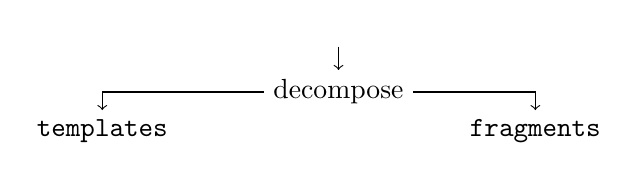
\begin{tikzpicture}[node distance=2cm]
% nodes
\node (Q) at (3, 1.2) {};
\node (C) at (3, .5) {decompose};
\node (A) at (0, 0) {\tt templates};
\node (D) at (5.5, 0) {\tt fragments};

% arrows
\draw[->] (Q) edge (C);
\draw[->, to path={-| (\tikztotarget)}]
  (C) edge (A)
  (C) edge (D);
\end{tikzpicture}
\end{figure}

\begin{figure}[h!]
\vspace{-2.0em}
\begin{subfigure}{.64\columnwidth}
\begin{lstlisting}[basicstyle=\scriptsize\ttfamily,numbers=none,xleftmargin=0.7em,xrightmargin=0em]
function f(uint256 arg) public {(?{\color{dkgreen}\$1}?)}
\end{lstlisting}
\end{subfigure}\hspace{.5em}
\begin{subfigure}{.26\columnwidth}
\begin{lstlisting}[basicstyle=\scriptsize\ttfamily,numbers=none,xleftmargin=0.7em,xrightmargin=0em]
f(notfound);
\end{lstlisting}
\end{subfigure}

\begin{subfigure}{.64\columnwidth}
\begin{lstlisting}[basicstyle=\scriptsize\ttfamily,numbers=none,xleftmargin=0.7em,xrightmargin=0em]
function f((?{\color{dkgreen}\$1}?)) public {
    f(notfound);
} 
\end{lstlisting}
\end{subfigure}\hspace{.5em}
\begin{subfigure}{.26\columnwidth}
\begin{lstlisting}[basicstyle=\scriptsize\ttfamily,numbers=none,xleftmargin=0.7em,xrightmargin=0em]
uint256 arg
\end{lstlisting}
\vspace{1.5em}
\end{subfigure}

\begin{subfigure}{.64\columnwidth}
\begin{lstlisting}[basicstyle=\scriptsize\ttfamily,numbers=none,xleftmargin=0.7em,xrightmargin=0em]
function f(uint256 arg) public {
    f((?{\color{dkgreen}\$1}?));
} 
\end{lstlisting}
\end{subfigure}\hspace{.5em}
\begin{subfigure}{.26\columnwidth}
\begin{lstlisting}[basicstyle=\scriptsize\ttfamily,numbers=none,xleftmargin=0.7em,xrightmargin=0em]
notfound
\end{lstlisting}
\vspace{1.5em}
\end{subfigure}
\end{figure}

A ``decompose'' operation yields three \texttt{templates} in the left column
({\tt\color{dkgreen}\$1} are placeholders for future substitution) and extracts
three corresponding concrete \texttt{fragments}, shown in the right column. 
The ``decompose'' operation is done with \texttt{Comby}, which extracts concrete
values inside parentheses, braces, and square brackets (patterns
\texttt{(\$expr)}, \texttt{\{\$expr\}}, \texttt{[\$expr]} respectively). Note
that our approach can be customized to extract \emph{any} kind of syntactically
significant pattern and correspondingly decompose the input program; we simply
chose syntax that commonly delineates code blocks and expressions (i.e.,
parentheses and braces) since these exhibit interesting properties that
preserve structure (multiline statements, well-formed expressions) that go
beyond what string-level mutations identify.

We perform this decomposition for all programs in the corpus to obtain
templates and concrete fragments, which we then deduplicate. Once fuzzing, the
server generates an input program by selecting, uniformly at random, a template
and up to 10 program fragments and then substitutes all locations in the
template with program fragments. In essence, the server splices new inputs that
are likely to compose syntactically well-formed programs.

In addition to generating inputs, the server can also apply syntax-aware
\texttt{Comby} transformation rules, analogous to string-level mutation
operators. In practice, our server architecture adds considerable overhead (we
discuss this in Section~\ref{eval}) and is thus slow in applying
on-the-fly mutations, and in that sense less
appealing than the string-level mutation. Our
results in Section~\ref{eval} do show, however, that generative
syntax-aware input manipulation demonstrates compelling utility despite
incurring significant slowdown.\footnote{We are actively improving the tooling
architecture, a matter of engineering rather than
limitations on the inherent merits of the approach.}

\subsubsection{P(havoc) + P(text) + P(splice) = 1}

Our full implementation is based on Google's released code for the AFL
fuzzer, and available as an open source tool (that, to date, has 68
stars on GitHub, has been forked 7 times, and has external users who
make bug reports and queries to us).\footnote{Link omitted for
  blinding.}  The main change to AFL is the addition of code such as that shown in
Figure~\ref{fig:foperators}.  The new version (the ``AFL compiler
fuzzer'') can also call out to {\tt comby} to generate mutants.  Two
new command line parameters to AFL control the use of these features:
{\tt -1} determines the probability to generate a mutant using the
fast C string implementation (with a default value of 75\%), and {\tt -2} determines the probability
to call {\tt comby} to generate a mutant (with a default value of
0\%).  If these two parameters add up to less than 100\%, the
remainder of the time the usual stock AFL havoc mutation operators are
applied; by default, this happens 25\% of the time.

\section{Evaluation}
\label{eval}

We ran a series of controlled experiments to evaluate the effectiveness of two
strategies based on our approaches in Sections~\ref{strat-fast-string-level}
and~\ref{strat-syntax-aware} for improving on ``no-fuss'' compiler fuzzing. Our
main goal is to answer to what extent these low-effort strategies demonstrate
significant benefit in the domain of compiler fuzzing, and how they influence
fuzzer behavior and performance.

Section~\ref{exp-setup} describes our experimental setup.
Section~\ref{exp-results} summarizes our results, which compares our strategies
against stock AFL and AFL++ fuzzers on four actively-developed compilers. 

\subsection{Experimental Setup}
\label{exp-setup}

We evaluate on four compilers for languages Solidity,\footnote{https://docs.soliditylang.org/}
Move,\footnote{https://move-book.com/} and Fe\footnote{https://fe-lang.org/} (smart contract languages)
and the trending general-purpose language Zig.\footnote{https://ziglang.org}. 


\noindent
\textbf{Fuzzing strategies}

\noindent \textbf{Fuzzing trials and duration.} We ran 16 trials per fuzzing
strategy for each compiler to control for variability and randomness. A single
trial comprises 24 hours of fuzzing on a single core, starting from the initial input corpus.
% 16*3*24+16*4*24 = 2,688 hours 
We chose 24 hour trials because...
Our experiments represent 112 days of aggregate fuzzing and thus offer
substantive evidence of fuzzer performance for quickly surfacing bugs under our
``no-fuss'' strategies on our chosen compilers.


\noindent 
\textbf{Input corpora.} For solidity, all \texttt{.sol} files in
\texttt{test/libsolidity}. For Move, all \texttt{.diem} files in the
repository. For \texttt{Fe}, {\color{red} all \texttt{.fe} files in
repository}. AFL starts of preprocessing inputs based on coverage and ignores uninteresting ones. {\color{red} say how many for each proj}

For the template splicing technique, we start off with a noop input and
gradually generate \texttt{(template, fragment)} pairs, synthesized on-demand.
After generating pairs,wWe removed all large inputs in the \texttt{(template, fragment)} corpus (> 4KB). {\color{red} say how many of these}.

% Data lives here:
% Solidity: /home/rijnard/0-experiments-feb/sol-programs                         @ 686b62b585d686f08fe2f8d586b8474c133dce2f + cherry-pick
%           /home/rijnard/0-experiments-feb/comby-mutation-server/fragments
% Move:     /home/rijnard/0-experiments-feb/move-programs                        @ bfb6b09715894b3c436919bf2e718b6ae0fcba9f (double check)
%           /home/rijnard/0-experiments-feb/comby-mutation-server-move/fragments
% FE        /home/rijnard/0-experiments-feb/fe-programs                          @ 1ea2206e3d10e77163f1a01bee05088358d8ef23
%           /home/rijnard/0-experiments-feb/comby-mutation-server-fe/fragments


\subsection{Results}
\label{exp-results}

\begin{table*}
\centering
\begin{tabular}{llrrrrrrcr}
\toprule
                    \bf Project      & \bf Configuration                           & \mc{3}{c}{\bf Unique Bugs}        & \bf Avg Execs  & \bf Avg Paths    & \bf Avg Bitmap    & \mc{2}{c}{\bf Queue}            \\
                                     &                                             & Avg     & Min       & Max         & (Millions)     & (K)              & Cvg (\%)          & Compiles (K)     & Unique Errs \\
\midrule
                    \mr{4}{Solidity} & \tt \small      AFL-baseline                &  3.69   & 1         &  6          & 35.8           & 12.0             & 54.34\ph{a}       & 2.89             & ????          \\ 
                                     & \tt \small      AFL++ 3.15a                 &  5.63   & 1         & 10          & 56.9           &  8.8             & 20.58$^\dagger$   & 3.80             & ????          \\ 
                                     & \tt \small      text-mutation               &  7.81   & 7         & 11          & 30.3           & 14.3             & 55.65\ph{a}       & 5.48             & ????          \\ 
                                     & \tt \small      splice-mutation             & 11.81   & 7         & 14          & 16.0           & 16.8             & 57.33\ph{a}       & 5.24             & ????          \\ 
\midrule
                    \mr{4}{Move}     & \tt \small      AFL-basline                 & 7.19    & 6         & 8           & 56.9           & 4.9              & 63.23\ph{a}       &                  &               \\ 
                                     & \tt \small      AFL++ 2.54b                 & ????    & ?         & ?           & ????           & ???              & ?????             &                  &               \\ 
                                     & \tt \small      text-mutation               & 8.31    & 7         & 9           & 61.2           & 6.0              & 62.27\ph{a}       &                  &               \\ 
                                     & \tt \small      splice-mutation             & 6.06    & 5         & 7           &  7.2           & 5.0              & 63.18\ph{a}       &                  &               \\ 
\midrule
                    \mr{4}{Fe}       & \tt \small      AFL-baseline                & 6.56    & 5         & 7           & 24.5           & 3.5              & 27.91\ph{a}       &                  &               \\ 
                                     & \tt \small      AFL++ 2.64c                 & 6.44    & 5         & 8           & 22.6           & 3.4              & 27.76\ph{a}       &                  &               \\ 
                                     & \tt \small      text-mutation               & 6.50    & 5         & 7           & 17.9           & 3.3              & 27.84\ph{a}       &                  &               \\ 
                                     & \tt \small      splice-mutation             & 6.94    & 6         & 9           &  5.0           & 2.6              & 27.83\ph{a}       &                  &               \\ 
\midrule
                    \mr{3}{Zig}      & \tt \small      AFL-baseline                & ????    & ?         & ??          & 2.2            & 3.3              & 40.99\ph{a}       &                  &               \\ 
                                     & \tt \small      text-mutation               & ????    & ?         & ??          & 2.1            & 3.3              & 40.95\ph{a}       &                  &               \\ 
                                     & \tt \small      splice-mutation             & ????    & ?         & ??          & 1.3            & 3.9              & 41.82\ph{a}       &                  &               \\ 
\bottomrule
\end{tabular} 
        \caption{Main results. We fuzzed each project for 16 trials (24 hours per trial) in different configurations: \texttt{baseline-AFL}, \texttt{AF++},  \texttt{text-mutation}, and \texttt{splice-mutation}.
\texttt{baseline-AFL} is stock \texttt{AFL}; \texttt{AFL++} is a community-driven effort that enhances stock AFL. \texttt{text-mutation} applies mutation operators (textual find-replace patterns) with a probability of 75\% on every fuzzed input. Sock AFL manipulates the input witht the remainder, 25\% of the time. \texttt{splice-mutation} is a hybrid approach that (1) applies mutation operators as in \texttt{text-mutation} with probability 33\%; (2) synthesizes a syntax-aware input with template (splice) 33\% of the time, and (3) uses stock AFL for the remainding 34\%. {\color{red} TODO: summarize results once flush.}}
\label{tab:results}
\end{table*}




\section{Non-Experimental Fuzzing Campaigns:  Bugs Reported}

{\bf WE NEED A NICE TABLE OF BUG CATEGORIES FOR ALL THE CAMPAIGNS WE RAN, INCLUDING CAMPAIGN LENGTH}

Perhaps the most important evidence of the effectiveness of this approach is that we applied it to fuzzing the Solidity compiler for over a year, and in that time reported XX bugs that have been fixed.  Prior to and during our campaign, Solidity had been fuzzed heavily using AFL, by the developers and by external contributors.  Despite competing with the internal fuzzing team of the project and other developers, and never devoting more resources to the fuzzing than 3-4 docker container hosted instances of our fuzzing tool, running on a high-end laptop, we believe that our campaign was the largest single source of fuzzing-discovered bugs in the compiler during our campaign.  The campaign was awarded a security bounty of \$1,000 USD in Ethereum for discovery of a bug with potential security implications (and, it was noted, for the general effectiveness of the fuzzing), and the Solidity team encouraged and aided our efforts, once it was clear that the approach was very useful in exposing subtle bugs.

A second long-term fuzzing effort was directed at the Fe language, a Rust/Python-like alternative to Solidity for writing Ethereum contracts.  Fe is an experimental language, and the project has far fewer resources than Solidity to devote to testing.  We worked with the Fe developers to make Fe crash in additional cases, and were able to provide them with high-quality fuzzing very early in the lifetime of an experimental compiler project.  We believe this effort was very useful to the Fe team, based on their comments, and speculate that better ``no-fuss'' fuzzing could expose language corner cases early in the implementation of a compiler, avoiding costly changes when more code depends on erroneous assumptions, or poor language design choices.

We also ran shorter, less-intensive campaigns against other compilers.
\section{Related Work}

Research on compiler testing, as noted in the introduction, has been an important subfield overlapping compiler development and design and software engineering and testing, for many years.  Chen et al. summarize much of this work in a recent survey~\cite{chen2020survey}.

To our knowledge, very little work has appeared targeting the problem this paper addresses: improving the ability of general-purpose fuzzers to find (interesting) bugs in compilers.  The recent work of Salls et al.~\cite{Salls2021TokenLevel}, however, specifically aims to improve general-purpose fuzzer performance on compilers and interpreters.  Their approach, which they call ``token-level fuzzing'' essentially produces a hybrid level in between grammar-based generation and ``byte-level'' mutation-based fuzzing.  The core of their idea is to replace the largely byte-level mutations of AFL etc. with mutations at the \emph{token} level of a grammar.  They summarize the idea as ``valid tokens should be replaced with valid tokens''~\cite{Salls2021TokenLevel}.  In a sense, this extends the idea of using a dictionary, but with important changes:  token-level fuzzing \emph{only} applies token-level, not byte-level mutations, but also adds the composition of multiple token additions and substitutions to the set of single-step mutations.  Token-level fuzzing is an attractive and useful idea, somewhat orthogonal to our approach.  However, unlike our approach, token-level fuzzing does not apply AFL's havoc operations, so some bugs are simply not possible to find using token-level fuzzing (e.g., ones involving injecting unprintable characters in strings, including our Solidity bug earning a security bounty).  In this sense, token-level fuzzing has some of the limitations of grammar-based generation.  Token-level fuzzing also provides little help to a fuzzer in deleting large chunks of code, since this often would require a very large number of token operations, though the approach does include a way to copy statements from one input to another.  Finally, token-level fuzzing requires using a lexer to find all tokens in input seeds, and if tokens not in those seeds would be useful, developers must provide any additional tokens.  This requires modifying the fuzzing workflow to add token pre-processing, and is no longer strictly \emph{no-fuss}.
\section{Conclusions}

Using automated methods to find bugs is an important part of modern
compiler development.  For a variety of reasons, the use of
off-the-shelf fuzzers, especially AFL, is the most widely used such
approach.  Mutation-based fuzzers, however, were originally used to
test binary formats, and their heritage limits their effectiveness for
fuzzing compilers.  Most solutions to this problem either place significant
burden on compiler developers, or are ineffective, or both.  We show
that using ideas from mutation testing it is possible to significantly
improve AFL-based fuzzing of compilers without forcing developers to
provide grammars or a dictionary.  One of our two configurations
performed best for all compilers we investigated, in experiments,
sometimes dramatically so (finding more than twice as many bugs on
average as the best version of un-augmented AFL).  Using our approach
we reported more than 100 previously unknown bugs, that have been
fixed as a result, in important
compiler projects.

{\small {\bf {Acknowledgements:}}  A portion of this work was supported by the National Science Foundation under CCF-2129446.}

\balance

\bibliographystyle{ACM-Reference-Format}
\bibliography{bibliography}

\balance

\end{document}
